\documentclass{article}


\usepackage{arxiv}
\usepackage[utf8]{inputenc} 	% allow utf-8 input
\usepackage[T1]{fontenc}    	% use 8-bit T1 fonts
\usepackage{hyperref}       	% hyperlinks
\usepackage{url}            		% simple URL typesetting
\usepackage{booktabs}       	% professional-quality tables
\usepackage{amsfonts}      	% blackboard math symbols
\usepackage{nicefrac}       	% compact symbols for 1/2, etc.
\usepackage{microtype}      	% microtypography
\usepackage{cite}
\usepackage{array}
\usepackage{multirow}
\usepackage{lipsum}
\usepackage{graphicx}

\title{Pre-flight Battery Consumption Model for UAV Missions}


\author{
  Eric R. Altenburg\\
  Computer Science\\
  Stevens Institute of Technology\\
  Hoboken, NJ \\
  \texttt{ealtenbu@stevens.edu}\\
   \And
  John H. Graves\\
  Computer Science\\
  Brown University\\
  Providence, RI \\
  \texttt{john\textunderscore graves@brown.edu} \\
  \And
  Qijun Gu\\
  Computer Science\\
  Texas State University\\
  San Marcos, TX \\
  \texttt{qg11@txstate.edu}\\
}


\begin{document}


\maketitle


\begin{abstract}
\lipsum[1]
\end{abstract}


% keywords can be removed
\keywords{Unmanned Aerial Vehicle \and UAV \and Drone \and Battery \and Battery Consumption \and Battery Usage \and Predict}


\section{Introduction}
In recent years, unmanned aerial vehicles (UAVs) have become increasingly popular in non-military contexts. As their technology improves, these devices become more and more integrated into society as they allow for tasks to be easily completed by a user in a remote location along a route. For example, Amazon and other distribution companies are developing methods that use these devices to deliver packages to their users in a fast and simple manner. As drones become more effective at delivering packages, they can replace trucks on short, relatively light deliveries, which will reduce the total amount of carbon dioxide emissions and have a positive impact on the environment \cite{Goodchild}. This technology is not limited to the aforementioned companies, instead, it is also used by archeological sites and other sports companies to conduct surveillance missions for certain dig sites where a camera might not be the best choice, or at a football game. Police forces also have begun to use these UAVs in situations where it is not entirely safe to send in an officer. By allowing that officer to remotely control a drone, it allows them and many others to be safe.\par

One of the many things holding UAVs back from doing such things is the simple fact that the battery usage is not easily predictable. By having the ability to know how much battery a given drone will consume can put the user at a much greater advantage as they can now determine whether or not a certain flight mission is feasible. Going back to the previous example with Amazon, their delivery drones may not always be charged to maximum capacity, therefore, if they can see how much battery a delivery will take up, then they can determine whether or not a different drone or a battery replacement will be required. Up until now, most UAV software can only communicate to the user how much battery is remaining in real time, and while that may be enough for most users, in some situations—like the one mentioned previously—it is important to know how much will be consumed before the UAV leaves the ground.\par

While there have been a few attempts at creating such a model, there has not been a successful method that results in an accurate or efficient prediction. This is partially due to drones being relatively new, having only been introduced in the past few years, and as a result, not much research has been conducted. It is from this lack of literature that many have had difficulty creating a functional model. Specifically, one of the assumptions made about these drones is that the total battery energy consumption is constant from flight-to-flight \cite{Prasetia}, however, through various data samples, this is not the case; it is variable. This and many other assumptions make up some of the shortcomings in existing literature, that if not proven correctly, can result in a considerable setback in the UAV field. 


\section{Related Work}
With very few pieces of literature in the spectrum of UAV battery consumption, there were a select few that stood out. Previous attempts at creating a similar model have attempted to separate the maneuvers a UAV performs during its flight into separate categories such as vertical, hover, and horizontal movements \cite{Prasetia}. Others took a more detailed approach and had back, down, forward, roll left, roll right, up, yaw left, and yaw right \cite{Corral}. Although these two studies were not entirely successful, they were still able to provide motivation to isolate the maneuvers into ascending, descending, hovering, and any horizontal movement.\par

As previously stated, these studies come with slight caveats. For the case of the detailed maneuver model, the data they collected on their quad-copter showed surprising results as shown in Figure 1. Here, they were able to map the current in Amps being drawn by each maneuver and deduced that down and roll left consumed little to no battery; up consumed the most; back, forward, roll right, yaw left, and yaw right consumed an amount in between the others. There are some aspects of this finding that raised concern, for example, roll left consumed a minuscule amount of current whereas roll right consumed much more. This puts roll left on the same level as moving down which seemed questionable. \par


\subsection{Improvements}
After collecting data from several flights, there was no similar pattern to that of their original findings, therefore, leading to the conclusion that roll left did not consume less power than roll right. Additionally, another finding in the data set showed that the differences in power consumption between all maneuvers in the horizontal plane were minute, thus allowing the classification of maneuvers to only include ascend, descend, hover, and horizontal movement. However, it is important to note that the UAV they used had four total rotors (quad-copter) while the one used primarily in this project had six rotors (hexa-copter) which could lead to a difference in results.


\section{Methods and Procedure}
One a very basic level, the model used two steps to predict pre-flight battery consumption. The first step was to determine which maneuvers a drone would fly. To do this, simulations were completed in the drone software QGroundControl and manually labeled with different maneuvers. This data was then used to train a machine learning model which could then take in a simulated projected flight path of an actual drone flight, and output a timeline of what maneuvers the drone would be doing and for how long.\par

The second modeling step was to predict the power associated with each maneuver, and ultimately the maximum flying battery life of a drone for a particular flight. First, five actual drone flights were manually categorized by maneuver, and analyzed to find the average power associated with each drone action. Next a separate series of tests were done with a grounded drone, draining the battery at different rates to test how much total energy the drone used before it dropped below the critical voltage level of 12V (citation?). A rational model was then fit to this data to predict maximum flight time of a drone given an average power during a flight.\par

Putting these parts together, the maximum flight time of a drone could be predicted by estimating how long the drone would be doing different maneuvers, using these durations and average power of maneuvers to determine an average power of the entire flight, and then using that number in the regression equation to predict the total flight time.


\subsection{Data Collection}
Three types of data were used for this model, each collected in their own separate way. First the machine learning model used simulation data for the QGroundControl software which simulates drone flights. The way this works is that a flight path with actions along the way is planned out, just as you would normally do pre-flight, but instead of going straight to doing the real test, this software can run a simulation before hand, included fairly detailed data about the position, rotation, acceleration, and speed of the drone. To train the machine learning model, ten tests were run in this simulation software, including a wide variety of paths and hovering at different altitudes. These paths included, squares, triangles, figure eights, simple straight paths, or just hovering in one spot the entire time. \par

The next type of data was the actual drone flights. The analysis relied on five different flights, taken at different times. Three of these flights had been recorded for a previous research project, but comprehensive data was available to analyze them. Two more of these flights were completed specifically for this research. One featured hovering for a minute at 20m and the other a clockwise circle at 10 m.\par

The third type of data collected was data from a grounded drone with its propellers flipped upside down to push it into the ground. With this setup, the drone would be put into manual mode and the throttle input was adjusted to test the results of draining the battery at different rates. The drone would be allowed to run until its voltage dropped into critical levels, the same level at which it would normally go into emergency landing procedure. One some of this data, the sensors stopped recording so power data could not be obtained, but in those cases total current draw was manual reported.


\subsection{Machine Learning}
In order to reduce the total amount of human error while evaluating maneuvers and streamline the overall process of estimating the battery consumption, machine learning proved to be a helpful tool. With the use of a classifier decision tree, the user would be capable of loading up simulation data from a desired flight plan, and the model will output a precise timeline of maneuvers the drone will perform every tenth of a second. As previously mentioned, this was a useful alternative to simply evaluating a flight pattern by eye as having the maneuvers of a drone off by a couple seconds could result in immensely different results when in practice. \par

The process of choosing this model was done so by evaluating what was needed for this project. Seeming as though there was no need for regression, it was clear that a model that worked with classification had to be used. While this narrowed the overall amount of options to choose from, there were still quite a bit left. Originally, random forests were set to be implemented, however, they tend to be costly in terms of time, and with the data smoothing algorithm that will be evaluated later on, speed was a concern. Finally, a decision tree was settled on due to its speed, easiness to understand, and favorable accuracy results. The entire tree was based on the Gini index–the probability of whether a decision is wrong or not, therefore, generally as one traverses farther down the tree, the Gini index should become smaller. An example of the tree can be seen in figure XX in which it shows a tree with a depth of XX. Generally speaking, finding the right depth of a tree depends entirely on the data as one does not want to over or under fit the data which will yield sub par results. \par


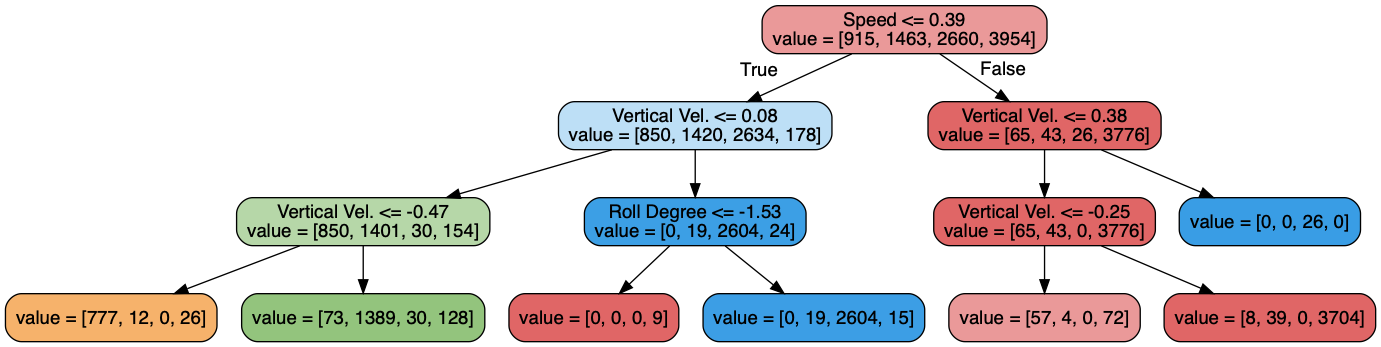
\includegraphics[scale = 0.25]{images/tree}

After the model is finished with all of its predictions, it outputs them all into a standard array, and once a simple compression algorithm is completed (see section XX) the timeline resembles one similar to figure XX. This however is still not the final result as there are still instances of sporadic predictions with a time value less than 10 (1 second). To correct this, a data smoothing algorithm is then applied (see section XX) where it will evaluate each maneuver to see whether it is below the 10 time unit threshold. If it is, it will then look above and below to determine which value to change it to; the maneuver will default to the one with the highest time value. The final result is then parsed to a comma-separate values (CSV) file where it will be used in average power prediction. An example of a final timeline can be seen in figure XX.


\subsection{Power Statistics}
To examine the average power of different maneuvers, the five five drone flights were manually divided up into sections representing the four maneuvers that were used in the machine learning model, by looking at altitude and ground speed. The data was reduced to one second intervals using the pchip method in matlab and then further smoothed by using a moving mean algorithm covering nine seconds (four on each side of the data point). \par

As Figure B shows, comparing the data from a single maneuver, in this case hovering, shows that there are large differences between these tests. This was explainable by different configurations in the drone, including parameters, settings, and even different copies of the same type of drone and battery. Of the five flights, flight one, flights two and three, and flights four and five were all under the same conditions, so the flights were separated into those three groups. A weighted average of power for each group of flights was preformed, which controlled for the frequency of different maneuvers. It did this by weighting each maneuver with a weight proportional to the smaller duration of that maneuver between the two flight groups being compared. Figure C shows this process with real data. By finding the ratio of these weighted averages, a coefficient was found to scale the power data from the first two groups of flights, which put them on par with the average power of group three. The normalized data was then analyzed with a box plot split by maneuver and by finding the average power of each maneuver to use in the final model. \par

To examine the maximum flight time the data from the grounded tests which drained the battery were parsed to find the total energy of each flight and the average power of each flight. For flights where the  sensors stopped recording mid-test, the total current draw was recorded and the relationship between total current and total energy was analyzed with linear regression to attempt to find a power approximation from these flights, even though the actual metric was not recorded. While processing this data it was noticed that the total energy of these flights was not constant as previous battery analysis had assumed (CITE), so further analysis was done to compare the total energy consumption of a test with its average power.


\section{Results and Discussion}


\subsection{Machine Learning}


\subsection{Power Statistics}


\section{Conclusion}


\section{LaTex Examples}
\label{sec:headings}

\subsection{Previous Research}
Previous research \par
Equation Example: \newline

\begin{equation}
\xi _{ij}(t)=P(x_{t}=i,x_{t+1}=j|y,v,w;\theta)= {\frac {\alpha _{i}(t)a^{w_t}_{ij}\beta _{j}(t+1)b^{v_{t+1}}_{j}(y_{t+1})}{\sum _{i=1}^{N} \sum _{j=1}^{N} \alpha _{i}(t)a^{w_t}_{ij}\beta _{j}(t+1)b^{v_{t+1}}_{j}(y_{t+1})}}
\end{equation}


\paragraph{Paragraph}
The Mentioned paragraph continues onto muliple lines it is a paragraph after all. What else do I write? I don't know


\label{sec:others}
When you have a paragraph you can also cite it. \cite{Prasetia} and see \cite{Chen} and see \cite{Corral}.

And for a URL, the documentation for \verb+natbib+ may be found at
\begin{center}
  \url{http://mirrors.ctan.org/macros/latex/contrib/natbib/natnotes.pdf}
\end{center}
Of note is the command \verb+\citet+, which produces citations
appropriate for use in inline text.  For example, 
\begin{verbatim}
   \citet{hasselmo} investigated\dots
\end{verbatim}
produces
\begin{quote}
  Hasselmo, et al.\ (1995) investigated\dots
\end{quote}

\begin{center}
  \url{https://www.ctan.org/pkg/booktabs}
\end{center}


\subsection{Figures}
See Figure \ref{fig:fig1}. Here is how you add footnotes. \footnote{Sample of the first footnote.}
See Section \ref{sec:headings}.

\begin{figure}
  \centering
  \fbox{\rule[-.5cm]{4cm}{4cm} \rule[-.5cm]{4cm}{0cm}}
  \caption{Sample figure caption.}
  \label{fig:fig1}
\end{figure}


\subsection{Tables}

See awesome Table~\ref{tab:table}.

\begin{table}
 \caption{Sample table title}
  \centering
  \begin{tabular}{lll}
    \toprule
    \multicolumn{2}{c}{Part}                   \\
    \cmidrule(r){1-2}
    Name     & Description     & Size ($\mu$m) \\
    \midrule
    Dendrite & Input terminal  & $\sim$100     \\
    Axon     & Output terminal & $\sim$10      \\
    Soma     & Cell body       & up to $10^6$  \\
    \bottomrule
  \end{tabular}
  \label{tab:table}
\end{table}


\bibliography{references}
\bibliographystyle{ieeetr}


\end{document}



